\documentclass{article}[12pt]
\setlength{\parskip}{\baselineskip}
\setlength{\parindent}{0pt}

\renewcommand{\baselinestretch}{1.5}

\usepackage[affil-it]{authblk}
\usepackage[space]{grffile}

\usepackage[a4paper]{geometry}
\usepackage[dvipsnames]{xcolor}
\geometry{verbose}

\usepackage{float}
\usepackage{graphicx}
\graphicspath{{figures/}}

\usepackage{setspace}
\usepackage{caption}

\usepackage[utf8]{inputenc}
\usepackage[english]{babel}

\usepackage{latexsym,textcomp,longtable,tabulary}
\usepackage{booktabs,array,multirow,braket}
\usepackage{amsfonts,amsmath,amssymb,mathbbol,calc}
\usepackage{subfigure,color,blindtext,enumitem,siunitx}
\usepackage[colorinlistoftodos]{todonotes}

\usepackage{mathtools}
\usepackage{url,hyperref,etoolbox}
\numberwithin{equation}{section}
\hypersetup{colorlinks=false,pdfborder={0 0 0}}

%+figure layout options
\restylefloat{figure}
\setlist{leftmargin=*,before=\setlength{\rightmargin}{\leftmargin}}
%-figure layout options

\providecommand\citet{\cite}
\providecommand\citep{\cite}
\providecommand\citealt{\cite}

\makeatletter
\makeatother

\begin{document}

\title{
Changepoint detection in an\\orchestra of musical instruments
}

\author{Student 1118161}
\affil{King's College London}
\date{\today}
\maketitle
\vspace{-3em}
\abstract{
\noindent
Music information retrieval tasks serve as faithful benchmarks for
time-series analysis pipelines due to the availability of strongly labelled
training data such as MusicNet. Q peak detection algorithm on a hand-crafted feature,
hidden Markov models and causal convolutional neural networks are compared in
their ability to detect changepoints in recordings of eleven orchestral instruments.
Detections are evaluated quantitatively with precision-recall metrics.}
\begin{figure}[H]
\centering{}
\captionsetup{justification=centering}
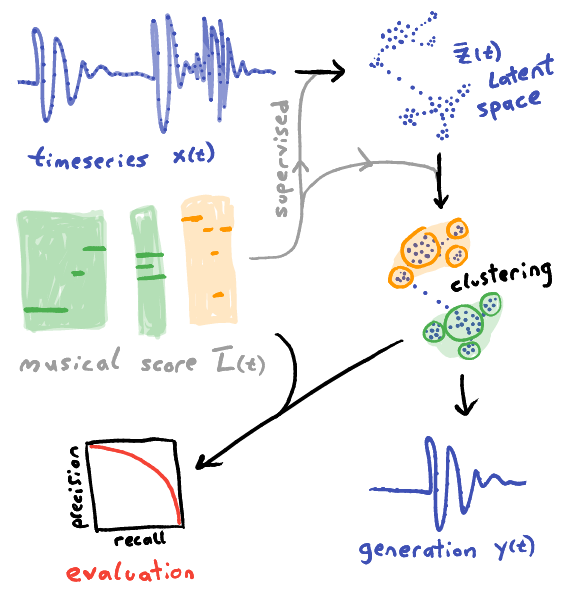
\includegraphics[scale=0.5]{methods}
\caption{Summary of methodology showing all stages of the audio segmentation task.\\
Each transition between sub-figures can be achieved with appropriate algorithms
}
\label{fig:methods}
\end{figure}
\section{Methodology Outline}
\subsection{Mapping time-series to latent space}
The input data are single channel time-series points $\mathcal{D}=\{x(t_1)\dots
x(t_N)\}$ sampled at frequency $f$ from an underlying continuous state-time
process $x(t)$, that is the oscillating sound waves emitted by a live orchestra.
\\\\
For each time point there is a polyphonic score matrix $\mathbf{L}(t)\in\{0,1\}^{N\times L}$ which
representing the $N$ midi notes played by $L$ instruments. Instrument activations
$\bar{\mathrm{y}}(t)\in\{0,1\}^L$ and $N$ note activations
$\bar{\mathrm{n}}(t)\in\{0,1\}^N$ can be individually considered as well as only
changepoints between states.
\noindent
The most difficult task is to recover the polyphonic score matrix
$\mathbf{L}(t)\in\{0,1\}^{N\times L}$ from the input signal $x(t)$. The score matrix
is generally sparse as playing too many notes with too many instruments at the
same time sounds terrible. Sparse labels lead to sparse learning signals which
hamper the convergence of machine learning algorithms. Thus we first look to
recover changepoints and then the more densly labelled $\bar{\mathrm{n}}(t)\in\{0,1\}^N$
and $\bar{\mathrm{y}}(t)\in\{0,1\}^L$.
From this we attempt to recover the full matrix in post-processing.
\\\\
Within unsupervised methods this task is known as
under-determined blind source separation. When the number of input channels
equals to the number of sources this problem is fully determined and can be
solved using independent component analysis
\cite{Platt1995Information-MaximizationDeconvolution} and other algorithms
that search for sparse representations. Through the lens of supervised approaches
this problem can be seen as an audio segmentation task. In recent years
convolutional networks have demonstrated success in image segmentation \cite{},
whos architectures are adaptable to audio data.
\\\\
The principal assumption in this task is that $x(t)$ is a linear superposition
of sources and that in some latent space $\bar{\mathrm{z}}(t)$ these sources are
linearly separable. The optimal latent space mapping $f$ should minimise the
cost function $J[f]$, which in general is some norm $\left\lVert\,\right\rVert$
of the error subject to some complexity measure $S[f]$. The data in the latent
space should be separable by a suitable choice of unmixing matrix $\mathbf{W}$.
\begin{align}
	J[f]=\left\lVert\bar{\mathrm{y}}(t)-\mathbf{W}\,\bar{\mathrm{z}}(t)\right\rVert+S[f]
	\quad\text{where}\quad
	\bar{\mathrm{z}}(t) = f(x,t)\\
	\exists\,\mathbf{W},f\,:\,f=\underset{f'}{\mathrm{argmin}}\,J[f']
	\qquad\qquad\qquad
\end{align}
Note that the map $f$ is most likely not one-to-one respect to $t$. It is not a
single time point but a time window that encodes which instrument is being
played. While linear separability via $\mathbf{W}$ by is sufficient it is not
necessary; one could instead simply look for clusters.
\subsubsection{Wavelet transforms and spectral speed}
The naive approach would be to attempt to guess the mapping $f$ via suitable
phenomenological agruments. It is reasonable to suppose that one could separate
instruments based on their spectral signature at any moment in time. The decibel
spectrogram $S(\omega,t)$ is obtained by taking the $\log_{10}$ absolute value
of a short-time fourier transform.
\begin{align}
	S(\omega,t):=\log_{10}\left[\left|\,
	\int_{-\infty}^{\infty}\!
		x(\tau)\mathbb{e}^{-\mathbb{i}\omega \tau}h(\tau-t)
	\,\mathrm{d}\tau
	\,\right|\right]
\end{align}
A suitable window function $h(t)$ must be chosen; different choices lead to
different amounts of spectral leakage and time-frequency domain resolution
\cite{}. For demonstration purposes a 46ms wide Hann window is chosen with a
stride of 3ms, which is on the order of the shortest duration of a musical
sound.
\begin{figure}[H]
\centering{}
\captionsetup{justification=centering}
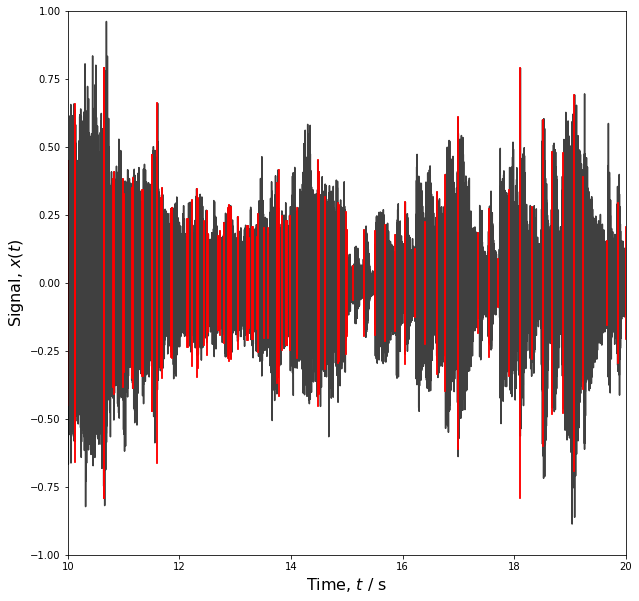
\includegraphics[scale=0.5]{signal}
\caption{
Input signal labelled with changepoints in polyphonic score $\mathbf{L}(t)$}
\label{fig:signal}
\end{figure}
\begin{figure}[H]
\centering{}
\captionsetup{justification=centering}
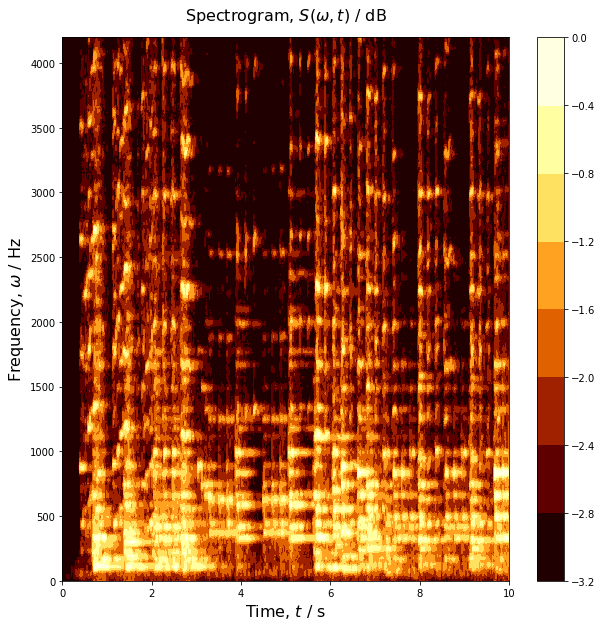
\includegraphics[scale=0.5]{spectrogram}
\caption{
Spectrogram $S(\omega,t)$ with dominant frequency labelled by instrument $\bar{\mathrm{y}}(t)$
}
\label{fig:spectrogram}
\end{figure}\noindent
The spectral signature of the input signal at a given time $t$ can be
represented as an $F$ dimensional point, where $F$ is the number
of frequency bins up to a given cutoff frequency calculated in the
spectrogram. The spectrogram in Figure \ref{fig:spectrogram} shows a
promising variety of signatures within domain $\Omega$ that may differentiate between instruments.
This observation motivates the calculation of spectral speed $v(t)$ defined as
\begin{align}
	v(t):= \frac{1}{|\Omega|}\int_{\Omega}\!\big|\partial_tS(\omega,t)\big|\,\mathrm{d}\omega
\end{align}
Figure \ref{fig:speed} reveals that peaks in spectral speed $v(t)$ typically
coincide with changepoints in notes and stepwise changes may indicate changepoints
in instruments. Peaks can be detected using wavelet transform approaches \cite{Du2006}
and true positives are counted when a detected peak lies within threshold time $\tau$
of a ground truth changepoint. Evaluations of 1000 clips of 5s from MusicNet
in Figure \ref{fig:pr} show that within 60ms a window approximately 60\% of the changepoints can be recalled with 60\% precision.
The duration of a quaver amongst Beethoven symphonies range 40-125ms. This suggests
that note changepoints more readily distinguised in slower symphonies. Such a claim
is supported by the example in \ref{fig:speed}, which shows a higher prevelance of
false positives and negatives in the fast paced signal on the left-hand side.
This approach is not precise enough to proceed with classification of the
segments between changepoints.

\begin{figure}[H]
\centering{}
\captionsetup{justification=centering}
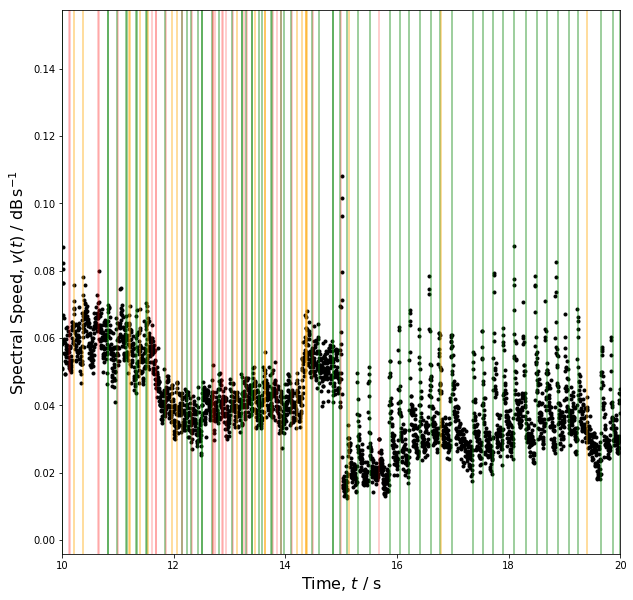
\includegraphics[scale=0.42]{detections}
\caption{
Spectral speed $v(t)$ labelled by $\color{Green}{\text{true positive}}$\\ $\color{orange}{\text{false positive}}$
and $\color{red}{\text{false negative}}$ changepoint detections
}
\label{fig:speed}
\end{figure}
\begin{figure}[H]
\centering{}
\captionsetup{justification=centering}
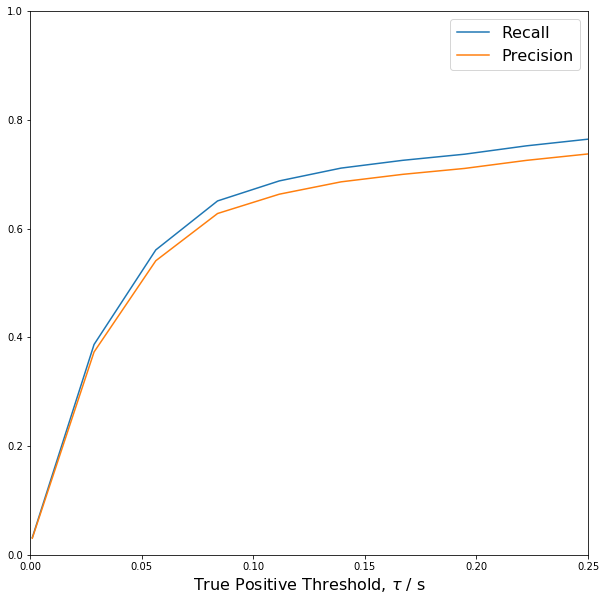
\includegraphics[scale=0.42]{pr}
\caption{
Changepoint precision-recall curves given by peaks in spectral speed $v(t)$
}
\label{fig:pr}
\end{figure}
\subsubsection{Markov models and expectation-maximisation} Hidden Markov models
with Gaussian mixture emissions have been successful in the first generation of
speech recognition piplines. Taking inspiration from these piplines, 11 separate
bimodal Gaussian models are fitted via expectation-maximisation to 11 separate datasets. Each dataset
contains 16 minute continuous concatinated spectrogram of a single instrument. Three
hidden states maximise the average likelihood of across models. The classification
of any new audio segment is given by the maximum likelihood model.
\\\\
Figure \ref{fig:confusion} shows classification results for 1000 clips each
lasting 100ms, whos ground truth labels are given by the dominant instrument in
the clip. With an average total accuracy of 73\% it outperforms the hand-crafted changepoint
classifier in Section 1.1.1. Changepoints are detected as the boundary between
any two classes, yielding the precision-recall curve in Figure \ref{fig:pr2}
\begin{figure}[H]
\centering{}
\captionsetup{justification=centering}
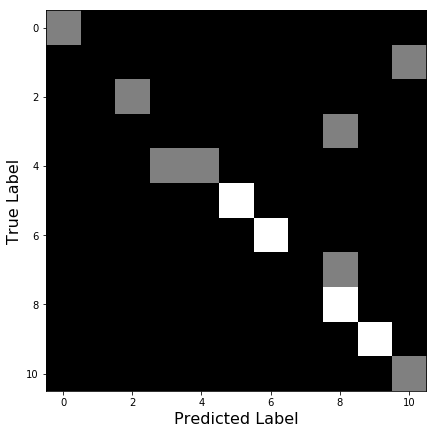
\includegraphics[scale=0.42]{confusion}
\caption{
Instrument confusion matrix given by maximum likelihood \\
Gaussian mixture Markov models for 100ms clip test set
}
\label{fig:confusion}
\end{figure}
\begin{figure}[H]
\centering{}
\captionsetup{justification=centering}
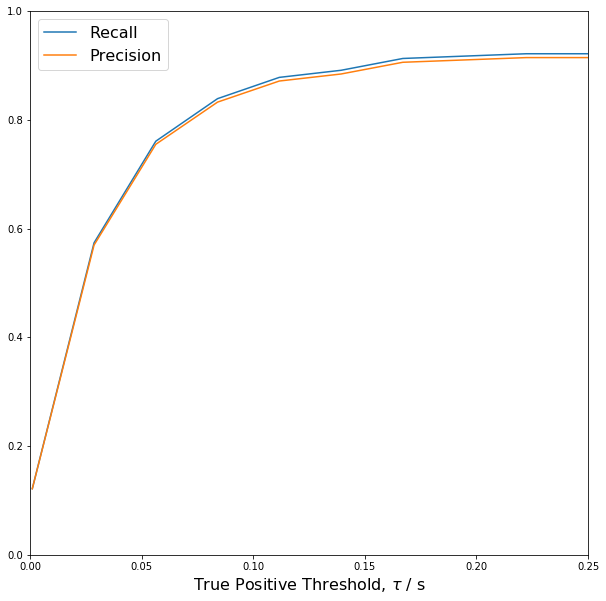
\includegraphics[scale=0.42]{pr2}
\caption{
Changepoint precision-recall curves given by classification boundaries of\\
maximum likelihood bimodal Gaussian mixture emissions Markov models
}
\label{fig:pr2}
\end{figure}

\subsubsection{Feature extraction with causal convolutions}
Convolutional architectures have become popular due to their ability to compress spatio-temporal
information for discrimination and generation tasks \cite{Oord2016a,Goodfellow}.
A causal convolutional network \cite{WaveNet} --- which encodes the arrow of time in
its architecture --- is trained for the audio segmentation task.
\\\\
Often the performance of the classifiers is hampered by poor choices of feature
space. Using the spectrogram as an input feature space in Sections 1.1.1 and
1.1.2 involves assumptions and arbitrary choices in the hyperparameters, such as
the shape of the wavelet window $h(t)$. Figure \ref{fig:wavenet} reveals a
schematic of the architecture of WaveNet, where the inputs are the audio samples
preceeding the next output sample. The arrow of time is encoded by the one-sided
convolutions and the dilated/downsampled layers serve to reduce dimensionality
and aggregate long range features in the waveform. In the original paper this
architecture was trained to generate the next audio sample, based on previous
samples. In our application we may ask for the instrument classification or
probability of changepoint as an output.
\begin{figure}[H]
\centering{}
\captionsetup{justification=centering}
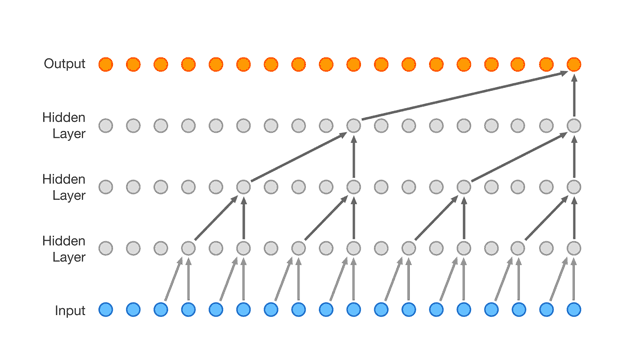
\includegraphics[scale=0.5]{wavenet}
\caption{
Causal convolutional architecture of WaveNet. Figure taken from \cite{WaveNet}
}
\label{fig:wavenet}
\end{figure}\noindent
Since this model takes the form of a computational graph, the back-propagation
algorithm can be used to train it. This algorithm has an intrinsic advantage over
expectation-maximisation as it can be optimally run on a GPU, which enables the
training on much larger datasets. Large test and training sets are necessary
for the models to generalise rather than overfit.
\\\\
\\\\
Due to time constraints and hardware limitations a smaller subset of MusicNet ---
1 minute per instrument --- was used as a training set to demonstrate overfitting.
A standard adaptive momentum gradient descent method \cite{Kingma2014} was used
and changepoints were detected as the boundary between any two classes on the same
test set as in Section 1.1.2. Figure \ref{fig:backprop} reveals the convergence
of the training protocol, giving rise to a very sensitive and nonspecific
changepoint classifier as shown by precision-recall curves in Figure \ref{fig:overfit}.
The relaively poor precision could be accounted for by the noisy classification
on the test set.
\begin{figure}[H]
\centering{}
\captionsetup{justification=centering}
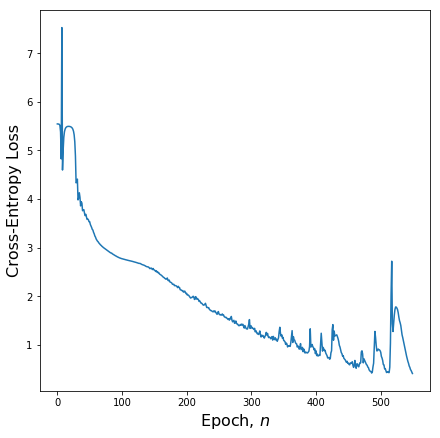
\includegraphics[scale=0.5]{backprop}
\caption{
Training loss as a function of ADAM epoch, showing convergence of WaveNet
}
\label{fig:backprop}
\end{figure}\noindent
\begin{figure}[H]
\centering{}
\captionsetup{justification=centering}
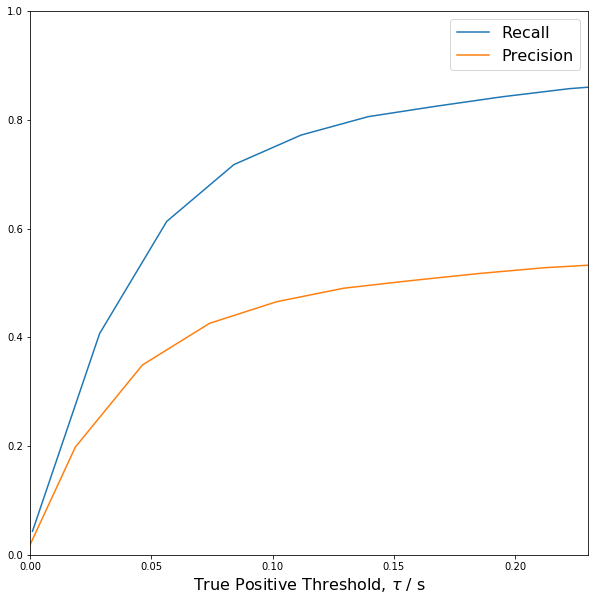
\includegraphics[scale=0.5]{overfit}
\caption{
Changepoint precision-recall curves given by classification boundaries of WaveNet
}
\label{fig:overfit}
\end{figure}

\bibliography{mendeley_v2}
\bibliographystyle{ieeetr}
\end{document}
